\documentclass[unicode,11pt]{beamer}
\usepackage{luatexja}
\usepackage[ipaex]{luatexja-preset}
\renewcommand{\kanjifamilydefault}{\gtdefault}


\usetheme{Madrid}

\title{中間発表}
\subtitle{最適配置問題へのPrincipal Pointsの応用}
\author{東京大学工学部計数工学科 数理情報コース4年\\梶山拳太郎}
\date{\today}
\institute{指導教員:松田孟留}

\begin{document}

\begin{frame}
    \titlepage
\end{frame}

\begin{frame}{今後の研究について:実データへの応用}
    \begin{itemize}
        \item 現在は日本の都市への施設配置問題に応用する予定.
        \item 東京のある都市における地域メッシュ統計による人口分布データをもとに2次元でのPrincipal Pointsを考え,施設配置を考える.
    \end{itemize}
    \begin{figure}[htbp]
        \begin{minipage}[b]{0.48\linewidth}
            \centering
            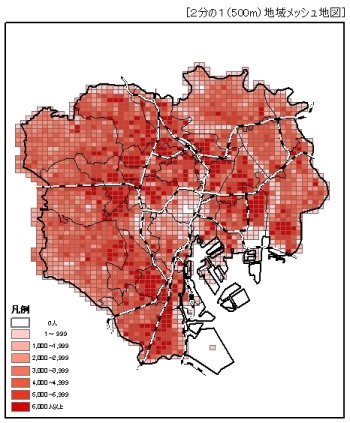
\includegraphics[keepaspectratio, scale=0.4]{tokyo_mesh_h22.jpeg}
            \caption{地域メッシュ統計(総務省統計局:「平成22年国勢調査に関する地域メッシュ統計」より引用)}
        \end{minipage}
        \begin{minipage}[b]{0.48\linewidth}
            \centering
            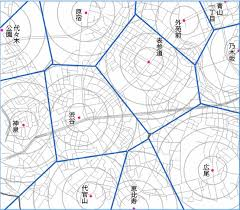
\includegraphics[keepaspectratio, scale=0.4]{voronoi_okabe.jpeg}
            \caption{地図上のボロノイ図(岡部篤行:第44回測量調査技術発表会「空間分析が歩んできた道,これから先の道」より引用)}
        \end{minipage}
    \end{figure}
\end{frame}

\begin{frame}{背景}
    \begin{itemize}
        \item Principal Pointsは[Flury,1990]より提案された.
        \item 与えられた確率分布の密度関数をk個の領域に分割する際の各領域の中心点と考えられる.
        \item 原論文では元々スイス軍の兵士向けに防護ヘルメットをなるべく頭のサイズにある最適なサイズで作成したいという動機から発展している.
    \end{itemize}
    \begin{figure}
        \centering
        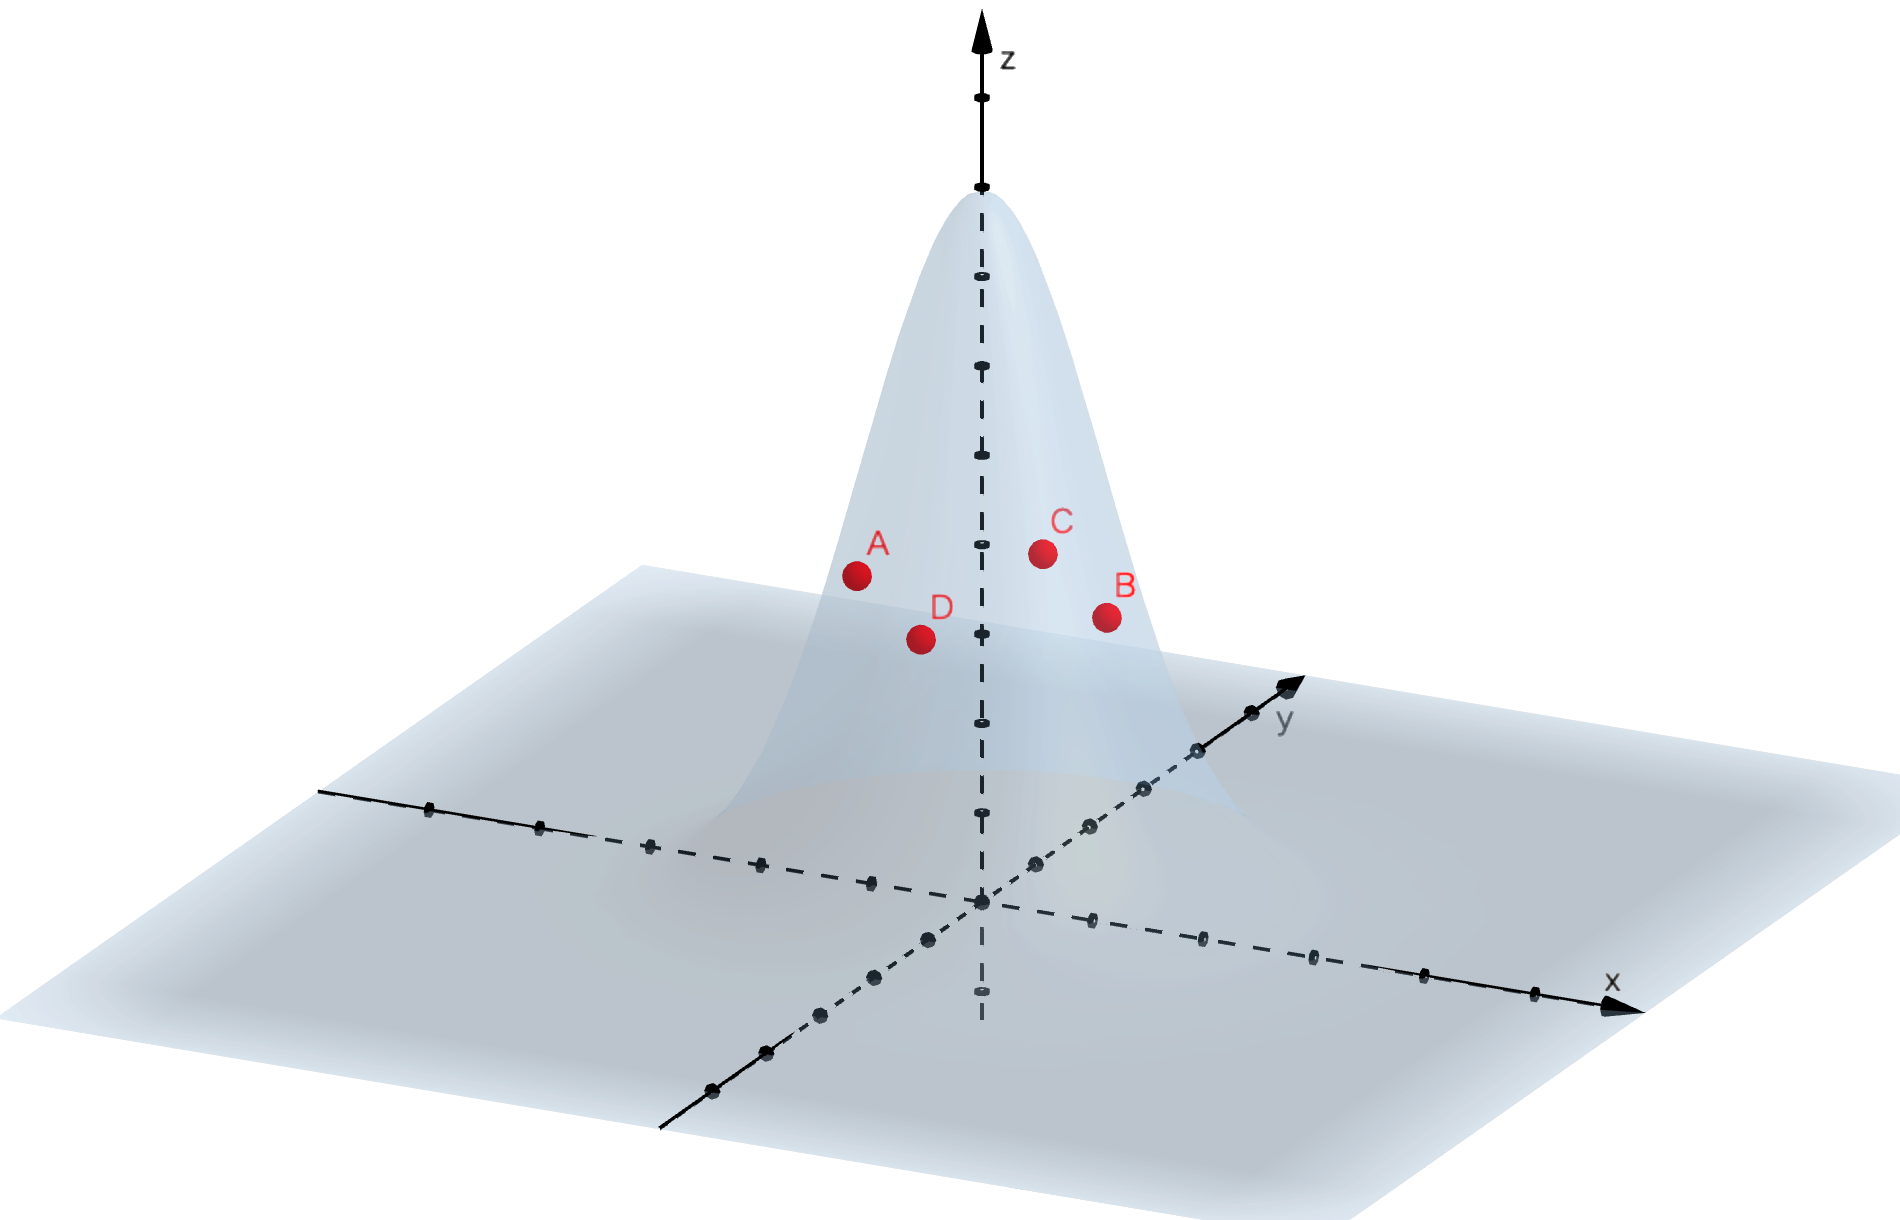
\includegraphics[keepaspectratio,scale = 0.2]{4-principal_points.png}
        \caption{標準正規分布の下での4-Principal Points}
    \end{figure}
\end{frame}

\begin{frame}{Principal Points}
    \begin{block}{k-Principal Points}
        $y_j \in R^p (1\le j \le k)$をp次元ユークリッド空間のk個の点とする.この時,$x \in  R^p$と$y_j (1 \le j \le k)$の距離は,
        \begin{equation}
            d(x|y_1,\dots,y_k) = \min_{1\le j \le k}{\{(x-y_j)'(x-y_j)\}}^{\frac{1}{2}}
        \end{equation}
        で定義される.\\
        この距離を利用してk-Principal Pointsは以下の等式を満たす$R^p$内の$k$個の点$v_1,v_2,\dots,v_k$で定義される.
        \begin{equation}
            E_F\{d^2(X|v_1,v_2,\dots,v_k)\} = \min_{y_j \in R^p, 1\le j \le k} E\{d^2(X|y_1,\dots, y_k)\}
        \end{equation}
    \end{block}
    クラスタリング手法において用いられることの多いk-means法と考える問題としては同じである.
    既存の手法としてはk-means法を考えることが多い.
\end{frame}

\begin{frame}{研究の方針}
    \begin{itemize}
        \item 距離の測り方$L_2$ノルムによる距離(ユークリッド距離)を用いた場合のPrincipal Pointsの性質、応用に関する研究が多い.
        \item 距離の測り方を変えた場合のPrincipal Pointsの性質,応用を考える.
        \item 別に既存手法の人口分布実データへの応用を考え,最適配置問題を考える.
    \end{itemize}
\end{frame}

\begin{frame}{距離の測定方法について}
    \begin{block}{Principal Points(再掲)}
        \begin{equation}
            E_F\{d^2(X|v_1,v_2,\dots,v_k)\} = \min_{y_j \in R^p, 1\le j \le k} E\{d^2(X|y_1,\dots, y_k)\}
        \end{equation}
    \end{block}

    \begin{block}{Principal Points(1次の場合)}
        \begin{equation}
            E_F\{d_1(X|v_1,v_2,\dots,v_k)\} = \min_{y_j \in R^p, 1\le j \le k} E\{d_1(X|y_1,\dots, y_k)\}
        \end{equation}
        ただし,
        \begin{equation}
            d_1(x|y_1,\dots,y_k) = \min_{1\le j \le k}{|x_j - y_j|}
        \end{equation}
    \end{block}
    2次の場合は各クラスターのデータの平均値を考えていたが,1次の場合には中央値を考えることになる.(Geometric Median)
\end{frame}

\begin{frame}{Geometric medianについて}
    \begin{columns}
        \begin{column}{0.48\textwidth}
            \begin{itemize}
                \item 1次の場合の1-Principal PointsはGeometric Medianと呼ばれる.
                \item アルゴリズムとして[Vardy \& Zhang,2000]の方法を採用する.
                \item 初期値をどこに決めても収束するという性質が優秀.
                \item 現行では4点の場合で考えると$d_2$距離を用いた場合と同様に対称性が見られる.
            \end{itemize}
        \end{column}
        \begin{column}{0.48\textwidth}
            \begin{figure}
                \centering
                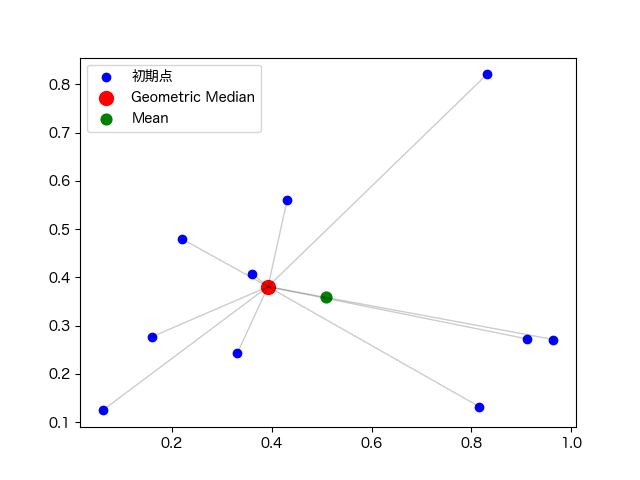
\includegraphics[keepaspectratio, scale = 0.7]{Geometric_Median.png}
                \caption{Geometric Median(Wikipedia:"Geometric Median"より引用}
                \label{Geometric_Median}
            \end{figure}
        \end{column}
    \end{columns}
\end{frame}

\begin{frame}{今後の研究について:距離の測り方について}
    $d_1$距離におけるPrincipalPointsの性質のさらなる追求
\end{frame}

\begin{frame}{今後の研究について:実データへの応用}
    \begin{itemize}
        \item [栗田,2004,2013]では東京の人口分布及びそれに伴う交通網は中心点(例,皇居)を基準に放射状に伸びていると考え,2次元→1次元の近似を行なって施設配置を考えている.
        \item こうした既存の結果と2次元データから考えた場合の配置とを比較,考察することも考えている.
    \end{itemize}
    \begin{figure}[htbp]
        \begin{minipage}[b]{0.45\linewidth}
            \centering
            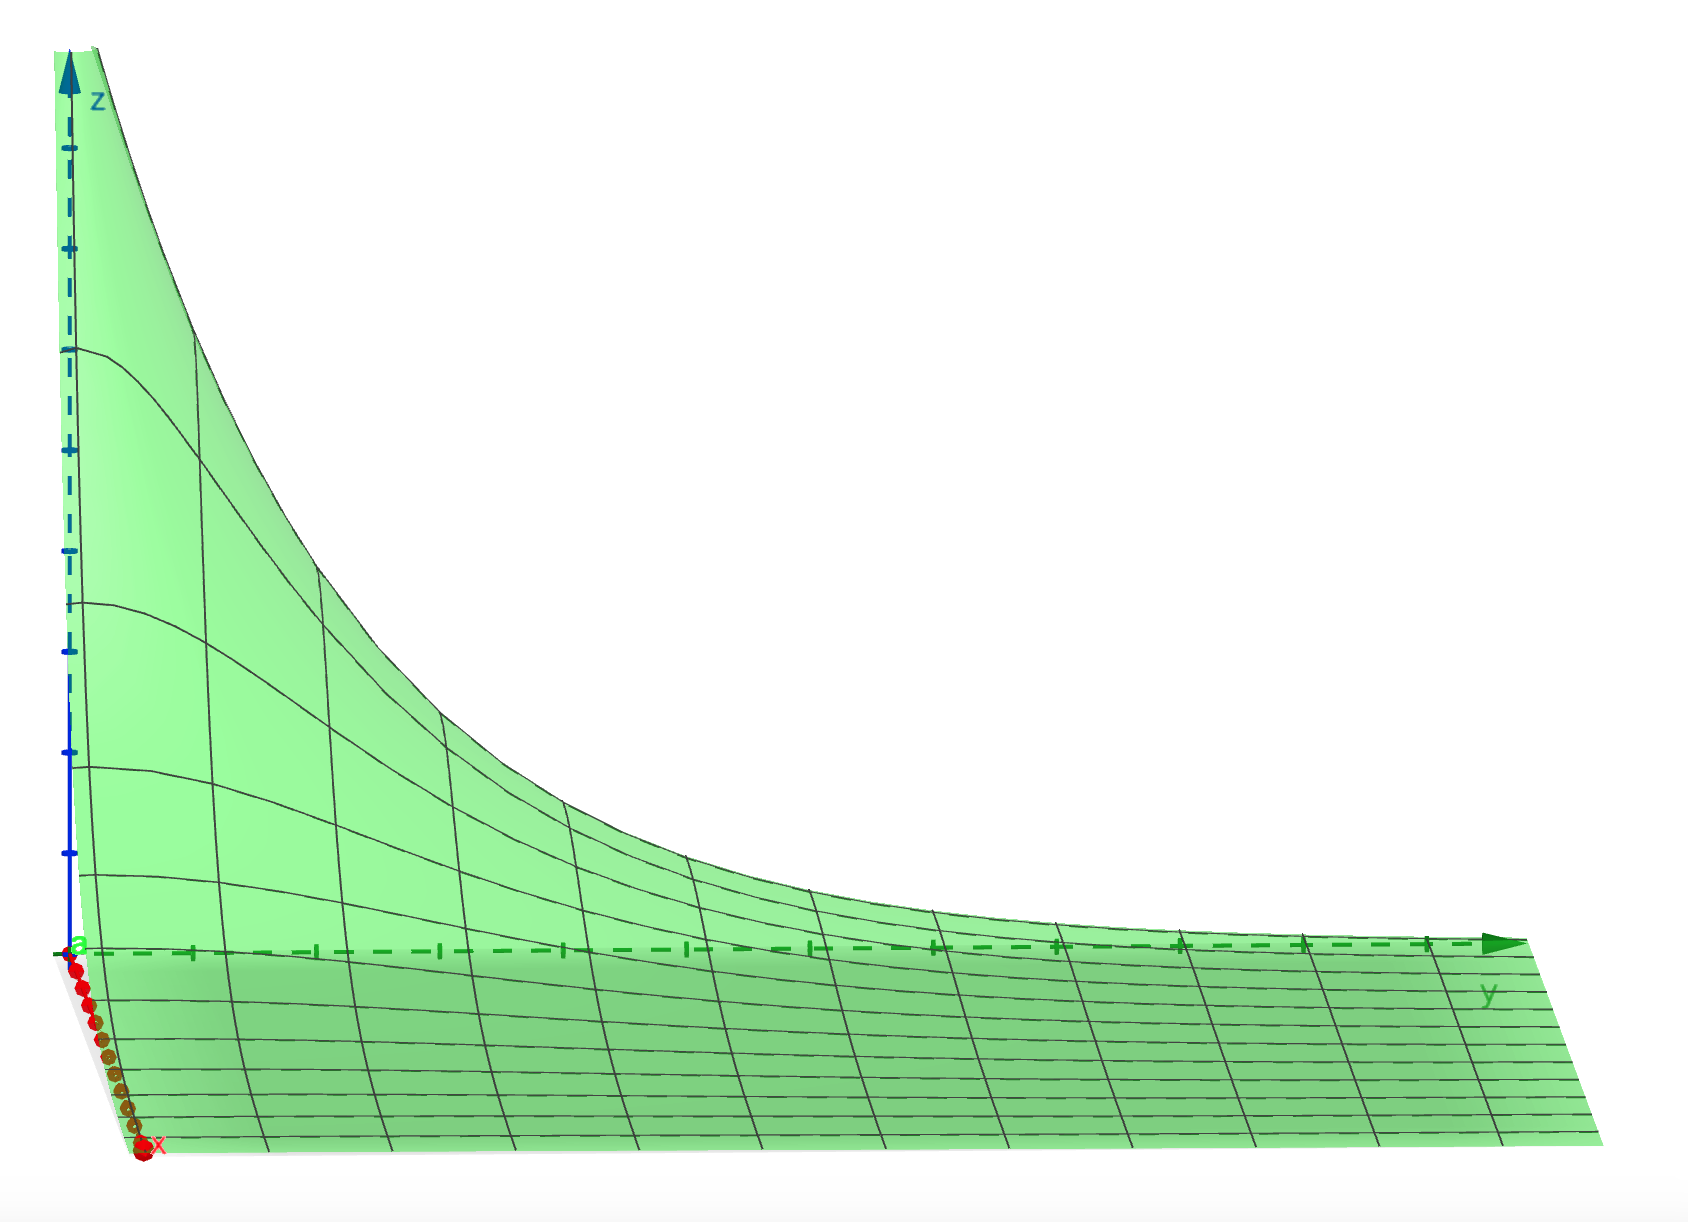
\includegraphics[keepaspectratio, scale=0.15]{z=e-u.png}
            \caption{回転対称な人口分布モデル}
        \end{minipage}
        \begin{minipage}[b]{0.45\linewidth}
            \centering
            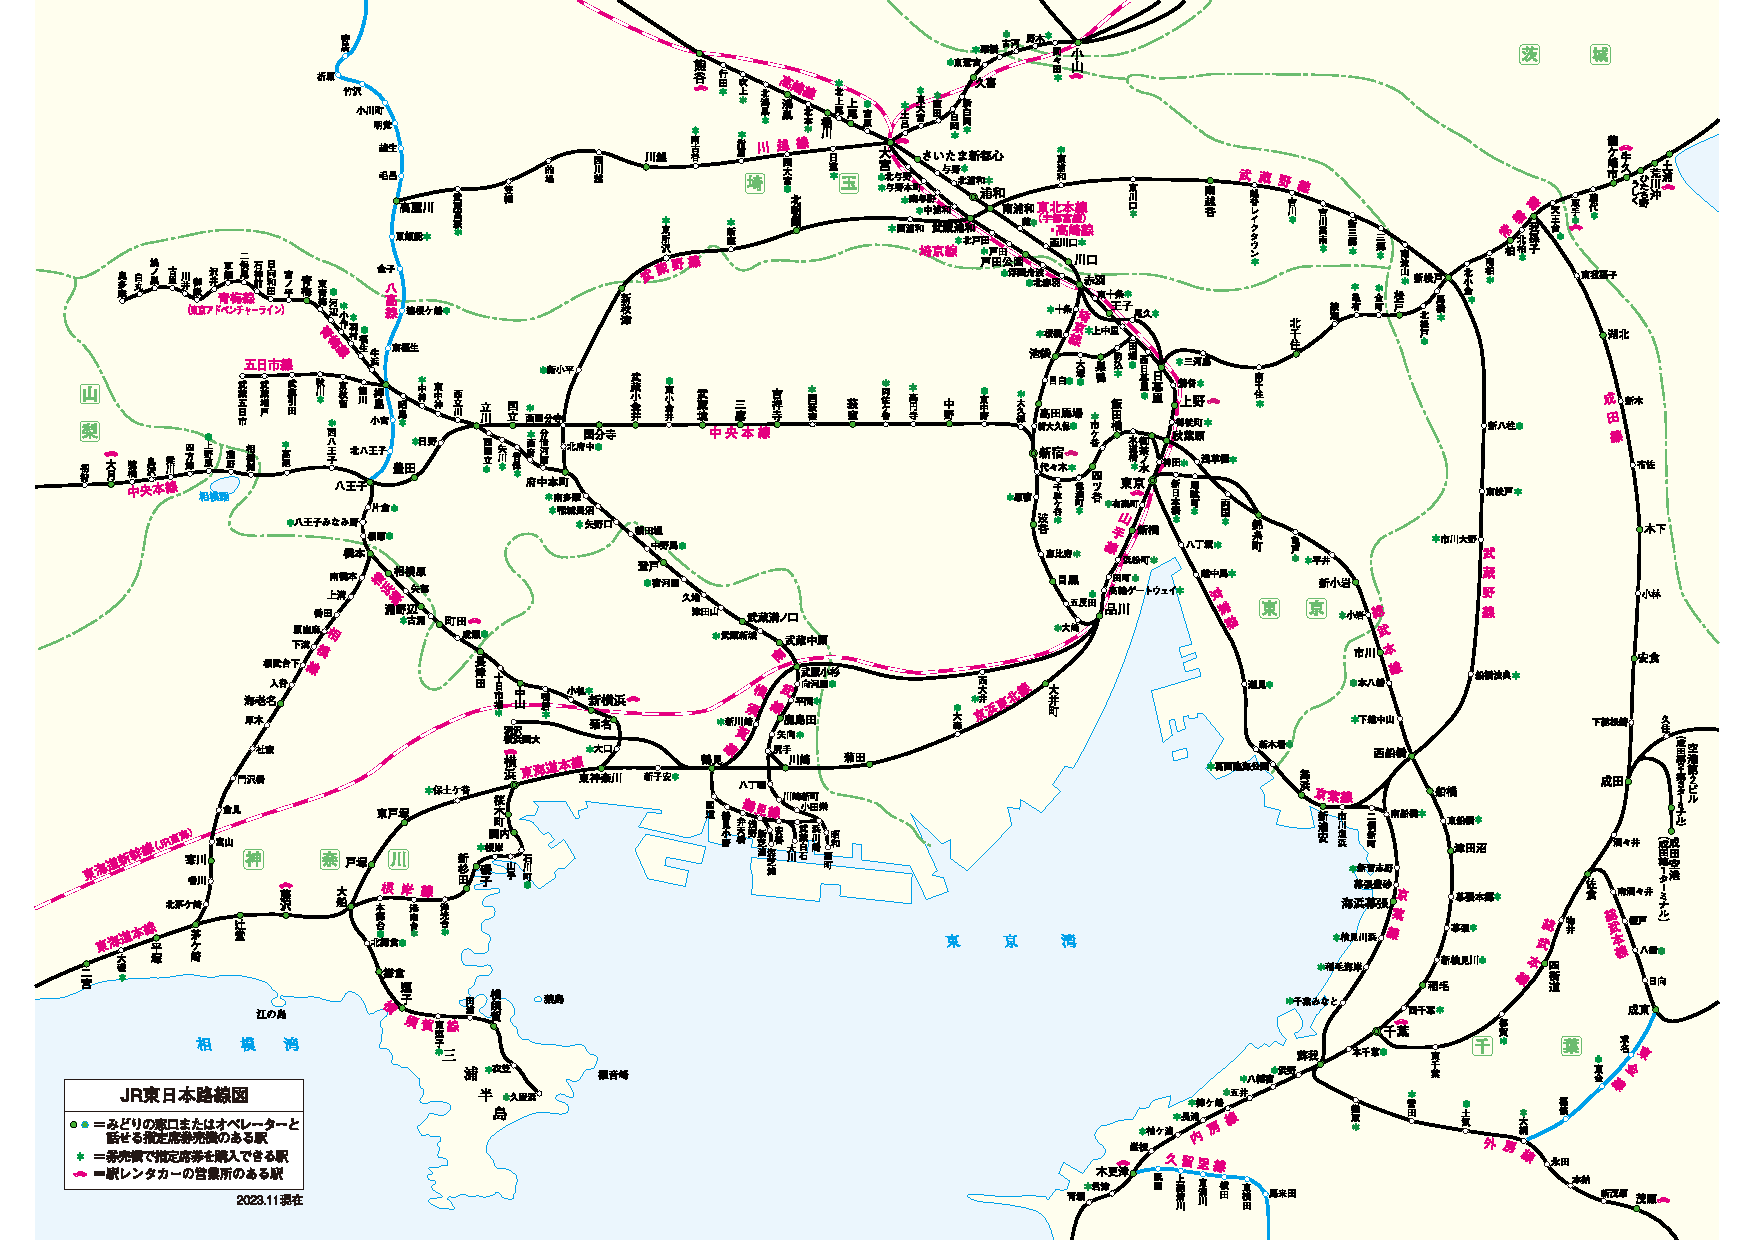
\includegraphics[keepaspectratio, scale=0.15]{tokyo.pdf}
            \caption{関東路線図(JR東日本:「路線図,東京近郊エリア」より引用}
        \end{minipage}
    \end{figure}
\end{frame}

\begin{frame}{参考文献}
    \begin{thebibliography}{99}
        \bibitem{Flury1990}Flury,B. Principal points. Biometrika. 1990, 77, 1, pp. 33-41.
        \bibitem{Flury1993}Flury,B. Estimation of Principal points. Journal of the Royal  Statistical Society. 1993, 42, 1, pp. 139-151.
        \bibitem{Shimizu}清水信夫,水田正弘,佐藤義治. Principal points の性質について. 応用統計学. 1998, 27, 1.
        \bibitem{Okabe}岡部篤行,鈴木敦夫 (1992). 最適配置の数理 ーシリーズ現代人の数理3ー. 朝倉書店
        \bibitem{Median_algorithm}Vardi,Y. \& Zhang, C-H. The multivariate $L_1$-median and associated data depth. Proceedings of the National Academy of Sciences of the United States of America. 2000, 97, 4, pp. 1423-1426.
        \bibitem{Kuritabook1}栗田治 (2013). 都市と地域の数理モデル. 共立出版.
        \bibitem{Kuritabook2}栗田治 (2004). 都市モデル読本. 共立出版.
    \end{thebibliography}
\end{frame}

\begin{frame}{参考文献}
    \begin{thebibliography}{99}
        \bibitem{Mesh}総務省統計局. ”平成22年国勢調査に関する地域メッシュ統計”. 総務省統計局. https://www.stat.go.jp/data/mesh/h22\_w.htm,(参照 2023-12-4).
    \end{thebibliography}
\end{frame}

\end{document}